\documentclass[letterpaper,12pt]{article}
\usepackage[margin=3.5cm]{geometry}
\usepackage[english]{babel}
\usepackage[utf8x]{inputenc}
\usepackage{amsmath}
\usepackage{graphicx}
\usepackage[colorinlistoftodos]{todonotes}
\usepackage{verbatim}

\title{IST557 Project 2}
\author{Sagnik Ray Choudhury, Wenyi Huang and Kyle Williams\footnote{Wenyi did experiments on decision tree, Kyle did experiments on pruning of the tree and Sagnik did experiments on random forest and boosting part. We all co-authored the report and slides together.}}

\begin{document}
\maketitle

\begin{abstract}
The author attribution problem involves determining whether or not an author wrote a paper. In this project, we compare the performance of decision tree, bagging and boosting methods for author attribution using data from the 2013 KDD Cup. 
\end{abstract}

\section{Introduction}
The author attribution problem involves determining whether a particular paper is written by a particular author and can be considered as a specific case of the author name disambiguation problem. At the KDD Cup in 2013, the task of author disambiguation was framed as a binary classification task where, given a set of [author, paper] pairs, the task was to classify the pair as positive (the author actually wrote that paper) or negative (the author didn't write that paper). We chose to address the same problem when investigating the use of different classification techniques as part of our class project.

From the given dataset described below (section \ref{sec:examples}), we extracted some features and investigated the use of decision trees with pruning, bagging and boosting. All our models were tested using 5-fold cross validation and the scikit-learn\footnote{http://scikit-learn.org} machine learning package was used for all experiments. Specifically: 
\begin{enumerate}
\item We evaluated different algorithms (original decision tree, pruning, bagging and boosting) on our dataset while allowing the tree to grow to unbounded depth. 
\item We systematically explored different depths of tree while making the decision tree classifer. We found that increasing the depth increases accuracy but increases model complexity as well. 
\item Using a fixed tree depth (which attributes to reasonable model complexity), we explored the effect of pruning, bagging and boosting. 
\item In the process of building trees with fixed length, we empirically validated that certain intuitive features actually work best for making splitting decisions.
\end{enumerate}

\section{Dataset}
\label{sec:examples}

\subsection{Original Dataset}
The following content is taken from KDD cup dataset page\footnote{http://www.kaggle.com/c/kdd-cup-2013-author-paper-identification-challenge} and presented with modifications as necessary. The provided datasets are based on a snapshot taken in Jan 2013 and contain:

An \textbf{Author dataset} (Author.csv) with profile information about 250K authors, such as author name and affiliation. The same author can appear more than once in this dataset, for instance because he/she publishes under different versions of his/her name, such as J. Doe, Jane Doe, and J. A. Doe. (see table \ref{table:author})

\begin{table}
\centering
  \caption{Author dataset}
\begin{tabular}{ |l |l |l |}
  \hline
  \textbf{Name} & \textbf{Data Type} & \textbf{Comments} \\ \hline
  Id & Int & Id of the author\\ \hline
  Name & NVarchar &  Name of the author\\ \hline
  Affiliation & NVarchar & Organization name with which the author is affiliated.  \\ \hline
\end{tabular}
\label{table:author}
\end{table}


A \textbf{Paper dataset} (Paper.csv) with data about 2.5M papers, such as paper title, conference/journal information, and keywords. The same paper may have been obtained through different data sources and hence have multiple copies in the dataset (see table \ref{table:paper}). 

\begin{table}
\centering
  \caption{Paper dataset}
\begin{tabular}{ |l |l |l |}
  \hline
 \textbf{Name} & \textbf{Data Type} & \textbf{Comments} \\ \hline
  Id & Int & Id of the paper \\ \hline
  Title & NVarchar &  Title of the paper\\ \hline
  Year & Int & Year of the paper  \\ \hline
  ConferenceId & Int & Conference Id in which paper was published\\ \hline
  JournalId & Int & Journal Id in which paper was published \\ \hline
  Keywords & Nvarchar & Keywords of the paper \\ \hline  
\end{tabular}
\label{table:paper}
\end{table}

A corresponding \textbf{Paper-Author dataset} (PaperAuthor.csv) with (paper ID, author ID) pairs. The Paper-Author dataset is noisy, containing possibly incorrect paper-author assignments that are due to author name ambiguity and variations of author names (see table \ref{table:paperauthor}).

\begin{table}
\centering
  \caption{Paper-Author dataset}
\begin{tabular}{ |l |l |l |}
  \hline
 \textbf{Name} & \textbf{Data Type} & \textbf{Comments} \\ \hline
  PaperId & Int & Paper Id\\ \hline
  AuthorId & Int & Author Id\\ \hline
  Name & Nvarchar & Author Name (as written on paper)\\ \hline
  Affiliation & Nvarchar & Author Affiliation (as written on paper)\\ \hline
\end{tabular}
\label{table:paperauthor}
\end{table}

Since each paper is either a conference or a journal, \textbf{additional metadata} (see table ) about conferences and journals is provided where available (Conference.csv, Journal.csv) (see table \ref{table:confjournal}).

\begin{table}
\centering
  \caption{Conference/Journal metadata dataset}
\begin{tabular}{ |l |l |l |}
  \hline
 \textbf{Name} & \textbf{Data Type} & \textbf{Comments} \\ \hline
  Id & Int & Conference Id or Journal Id \\ \hline
  ShortName & NVarchar & Short Name\\ \hline
  FullName & Nvarchar & Full Name\\ \hline
  HomePage & Nvarchar & Homepage URL of conf/journal \\ \hline
\end{tabular}
\label{table:confjournal}
\end{table}

\textbf{Co-authorship can be derived from the Paper-Author dataset}.


Papers that authors have confirmed (acknowledging they were the author) or deleted (meaning they were not the author) made up the data that we used for experimentation.

\section{Features}

For each ($a_i,p_j$) pair, where $a_i$ is the $i$-th author and $p_j$ is the $j$-th paper, we extracted the following features:
\begin{enumerate}
\item Number of papers $a_i$ has published in the journal $p_j$ was published in.
\item Number of papers $a_i$ has published in the conference $p_j$ was published in.
\item Number of papers $a_i$ has published.
\item Number of authors in $p_j$.
\item Suppose co-authors of $a_i$ for $p_j$ are $A_k | k \in (1:n)$. We created a vector P such that $P_{k}$= number of papers $a_i$ co-authored with $A_k$. We used sum, min, max, standard deviation and mean of the vector as separate features.
\item Suppose co-authors of $a_i$ for $p_j$ are $A_k | k \in (1:n)$. We created a coauthorship vector C where C[k]= Number of conferences/journals $a_i$ and $A_k$ published in together. We used mean, standard deviation, minimum, max and sum of this vector (C) as separate features.  
\end{enumerate}

Therefore, our feature space is 14 dimensional. 

\section{Experiments}
We conducted experiments to evaluate the performance of the decision trees under varying conditions for classifying the ($a_i, p_j)$ pairs. The first of these involved an unbounded tree that was allowed to grow as required followed by an experiment that investigated the effect of limiting the depth of the tree. We then evaluated the effect of pruning the tree and, lastly, we investigated the use of random forests. The total number of (author, paper) pairs that we had was 235,909 and for each experiment we evaluated the performance of our classifiers using 5-fold cross validation.

\subsection{Performance Metrics}
We employ the following performance metrics in our evaluation:

\begin{description}
\item[Accuracy:] the number of attributions correctly classified.
\item[Precision (sensitivity) (P):] the number of positive classifications that were truly positive. $\dfrac{tp}{tp+fp}$.
\item[Recall (R):] the number of truly positive classifications that were classified positive. $\dfrac{tp}{tp+fn}$.
\item[F1-score:] $\dfrac{2\cdot P \cdot R}{P + R}$
\end{description}

\subsection{Performance of Decision Trees}
\subsubsection{Unbounded Tree}\label{sec:unbounded}
Table \ref{performance} shows the performance of an unbounded decision tree that was allowed to grow as required. The parameters of this bounded tree are as follows:

\begin{itemize}
\item\textbf{Goodness of splits:} Gini \& entropy
\item\textbf{Stopping criteria:} All leaves are pure or until all leaves contain less than 2 samples.
\item\textbf{Class assignments:} 1 (author) or 0 (not author)
\end{itemize}

For this decision tree, the total number of nodes was approximately 30,000, approximate half of which were terminal nodes. As can be seen from the table, the the Gini and Entropy splitting criteria perform approximately the same achieving around 93\% for all performance metrics, with entropy performing slightly better than Gini as a splitting criterion. 


\begin{table}[h]
\centering
\caption{Performance of unbounded decision tree with different splitting criteria}\label{performance}
\begin{tabular}{|l|c|c|}
\hline
& Gini & Entropy\\\hline
Accuracy & 0.9282 & 0.9313\\\hline
Precision (sensitivity) & 0.9384 & 0.9409\\\hline
Recall & 0.9234 & 0.9270\\\hline
F1 & 0.9308 & 0.9349\\\hline
\end{tabular}
\end{table}

\subsubsection{Bounded Tree}
Since the unbounded tree became extremely large, we investigated the effect of limiting the depth of the tree. These bounded trees were defined as follows:

\begin{itemize}
\item\textbf{Goodness of splits:} Entropy
\item\textbf{Stopping criteria:} Depth of tree d={1,2,...,29}. All leaves are pure or until all leaves contain less than 2 samples.
\item\textbf{Class assignments:} 1 (author) or 0 (not author)
\end{itemize}

Figure \ref{fig:depth} shows the performance of the decision trees with varying depths. As can be seen from the figure, increasing the depth of the tree leads to an increase in accuracy, precision and the $F_1$ score. The recall jumps as the tree depth increases from 1 to 2, and then begins to decrease at a slow rate as the depth of the tree is increased. 

\subsubsection{Maximum Depth of Decision Tree}
\label{subsec:dectreemaxdepth}
For subsequent experiments with bounded depth trees, we choose a maximum tree depth of 10 as we found that this led to reasonable performance while reducing the model complexity and processing time.

\begin{figure}[ht!]
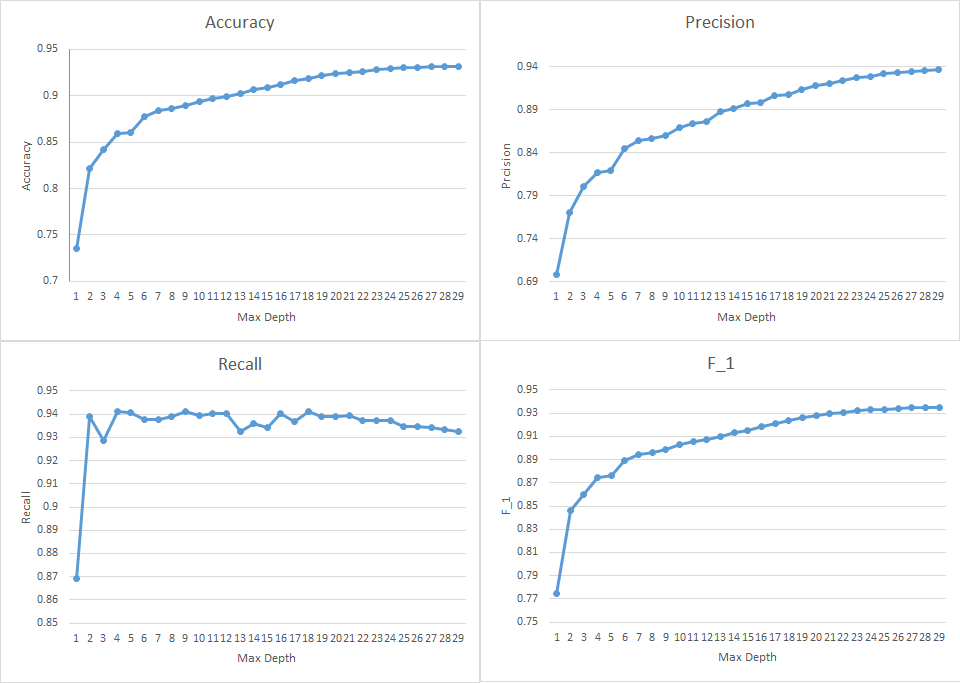
\includegraphics[width=\textwidth]{trees_result.png}
\caption{Performance when increasing the depth of the decision trees.}\label{fig:depth}
\end{figure}

\subsection{Tree Pruning}

We investigated the effect of pruning our trees. The pruning was done in such a way that we would grow a tree, select a max number of terminal nodes $m$, and then prune the tree by setting $m \leftarrow m -1$ with each iteration. This is a variation on the standard pruning algorithm where instead of growing the tree by adding new terminal nodes, we instead grow the full tree and then reduce the number of terminal nodes.

\textbf{Value of m}: In the unbounded case, there may be at most 236K terminal nodes (we do a 4:1 training:test data split with 293K data points). However, trying the iterative pruning process with more than 5000 terminal nodes is computationally too expensive, so we limit value of m to 5000.    

If we fix the depth of the tree to d, the number of leaf (terminal) nodes can be at most $2^{d-1}$ (as decision tree is a binary tree). As we choose d to be 10, a reasonable pruning bound is m=400. 

\subsubsection{Pruning of Unbounded Tree}

As mentioned before, for the unbounded tree, we set $m=5,000$ and the remaning parameters as follows:

\begin{itemize}
\item\textbf{Goodness of splits:} Entropy
\item\textbf{Stopping criteria:} All leaves are pure or until all leaves contain less than 2 samples.
\item\textbf{Class assignments:} 1 (author) or 0 (not author)
\end{itemize}

Figure \ref{fig:prune_unlimited} shows the effect of pruning on the performance of the unbounded tree. 

\begin{figure}[ht!]
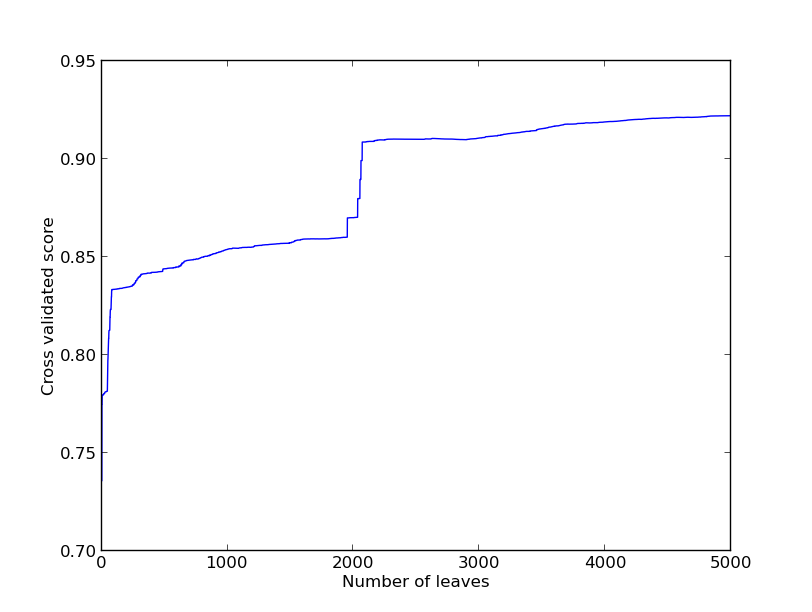
\includegraphics[width=\textwidth]{prune-unlimited.png}
\caption{Effect of pruning the unbounded decision tree.}\label{fig:prune_unlimited}
\end{figure}

As can be seen from the figure, there is no evidence of overfitting as increasing the number of terminal nodes always leads to an improvement in accuracy. Interestingly, from the figure it appears that at approximate 3,500 terminal nodes, the accuracy is very close to the 93\% accuracy achived by the unbounded tree with no pruning as described in Section \ref{sec:unbounded}.

\subsubsection{Pruning of Bounded Tree}
For the bounded tree we set $m=500$ and the remaining parameters as follows:

\begin{itemize}
\item\textbf{Goodness of splits:} Entropy
\item\textbf{Stopping criteria:} Max depth 10
\item\textbf{Class assignments:} 1 (author) or 0 (not author)
\end{itemize}

Figure \ref{fig:prune_10} shows the effect of pruning on the accuracy of the bounded tree.

\begin{figure}[ht!]
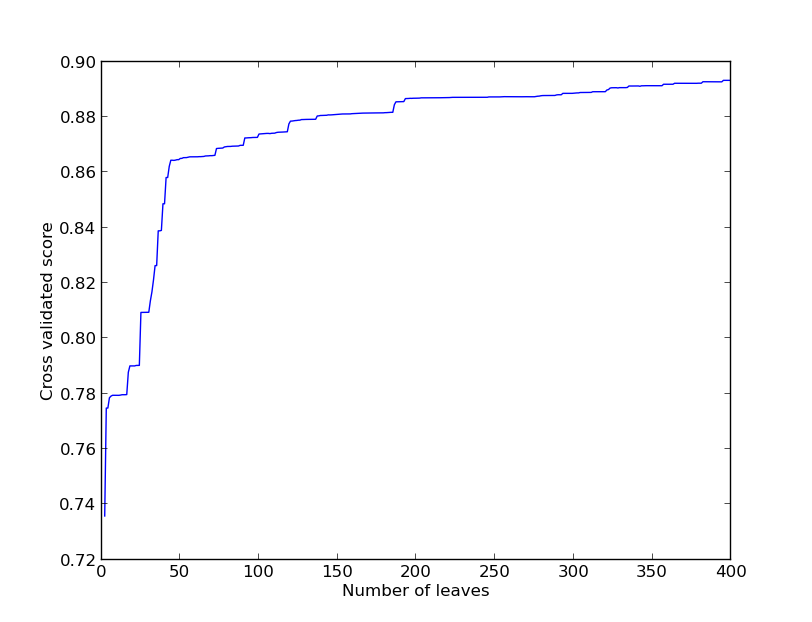
\includegraphics[width=\textwidth]{prune-depth10.png}
\caption{Effect of pruning the bounded decision tree.}\label{fig:prune_10}
\end{figure}

As can be seen from the figure, pruning has no effect on the performance of the decision tree and the accuracy increases as more leaves are allowed. From this it can be concluded that no over-fitting had occurred. It can also be seen from the figure that increasing the number of terminal nodes beyond 200 has little effect on the accuracy of the bounded decision tree.

\subsubsection{Analysis of a Pruned Tree}
Figure \ref{fig:tree} shows a pruned decision tree with 25 terminal nodes and a maximum depth of 10. As can be seen from the figure, the first split in our tree is on feature X[5]. For this split, $\frac{1}{3}$ of the data is immediately classified in a terminal node, whereas the other $\frac{2}{3}$ are further split for classification. Interestingly, when we set the depth of our tree to 1, this feature was able to achieve approximately 73\% classification accuracy. 

We explain the feature in details here. For a data point ($a_i, p_j$), we calculate number of times $a_i$ co-authors with the co-authors of $p_j$ and the minimum of that array. The splitting condition shows $a_i$ should have been a co-author with one of the authors of paper $p_j$ at least once before.

The other feature that is used for splitting these remaining $\frac{2}{3}$ of the data results in approximately 90\% of the data being classified at a terminal node. This feature captures the number of conferences the co-authors of the paper have published in together.

The remainder of the tree is then used for classifying the remaining 10\% of the data that appeared at that node.


\begin{figure}[ht!]
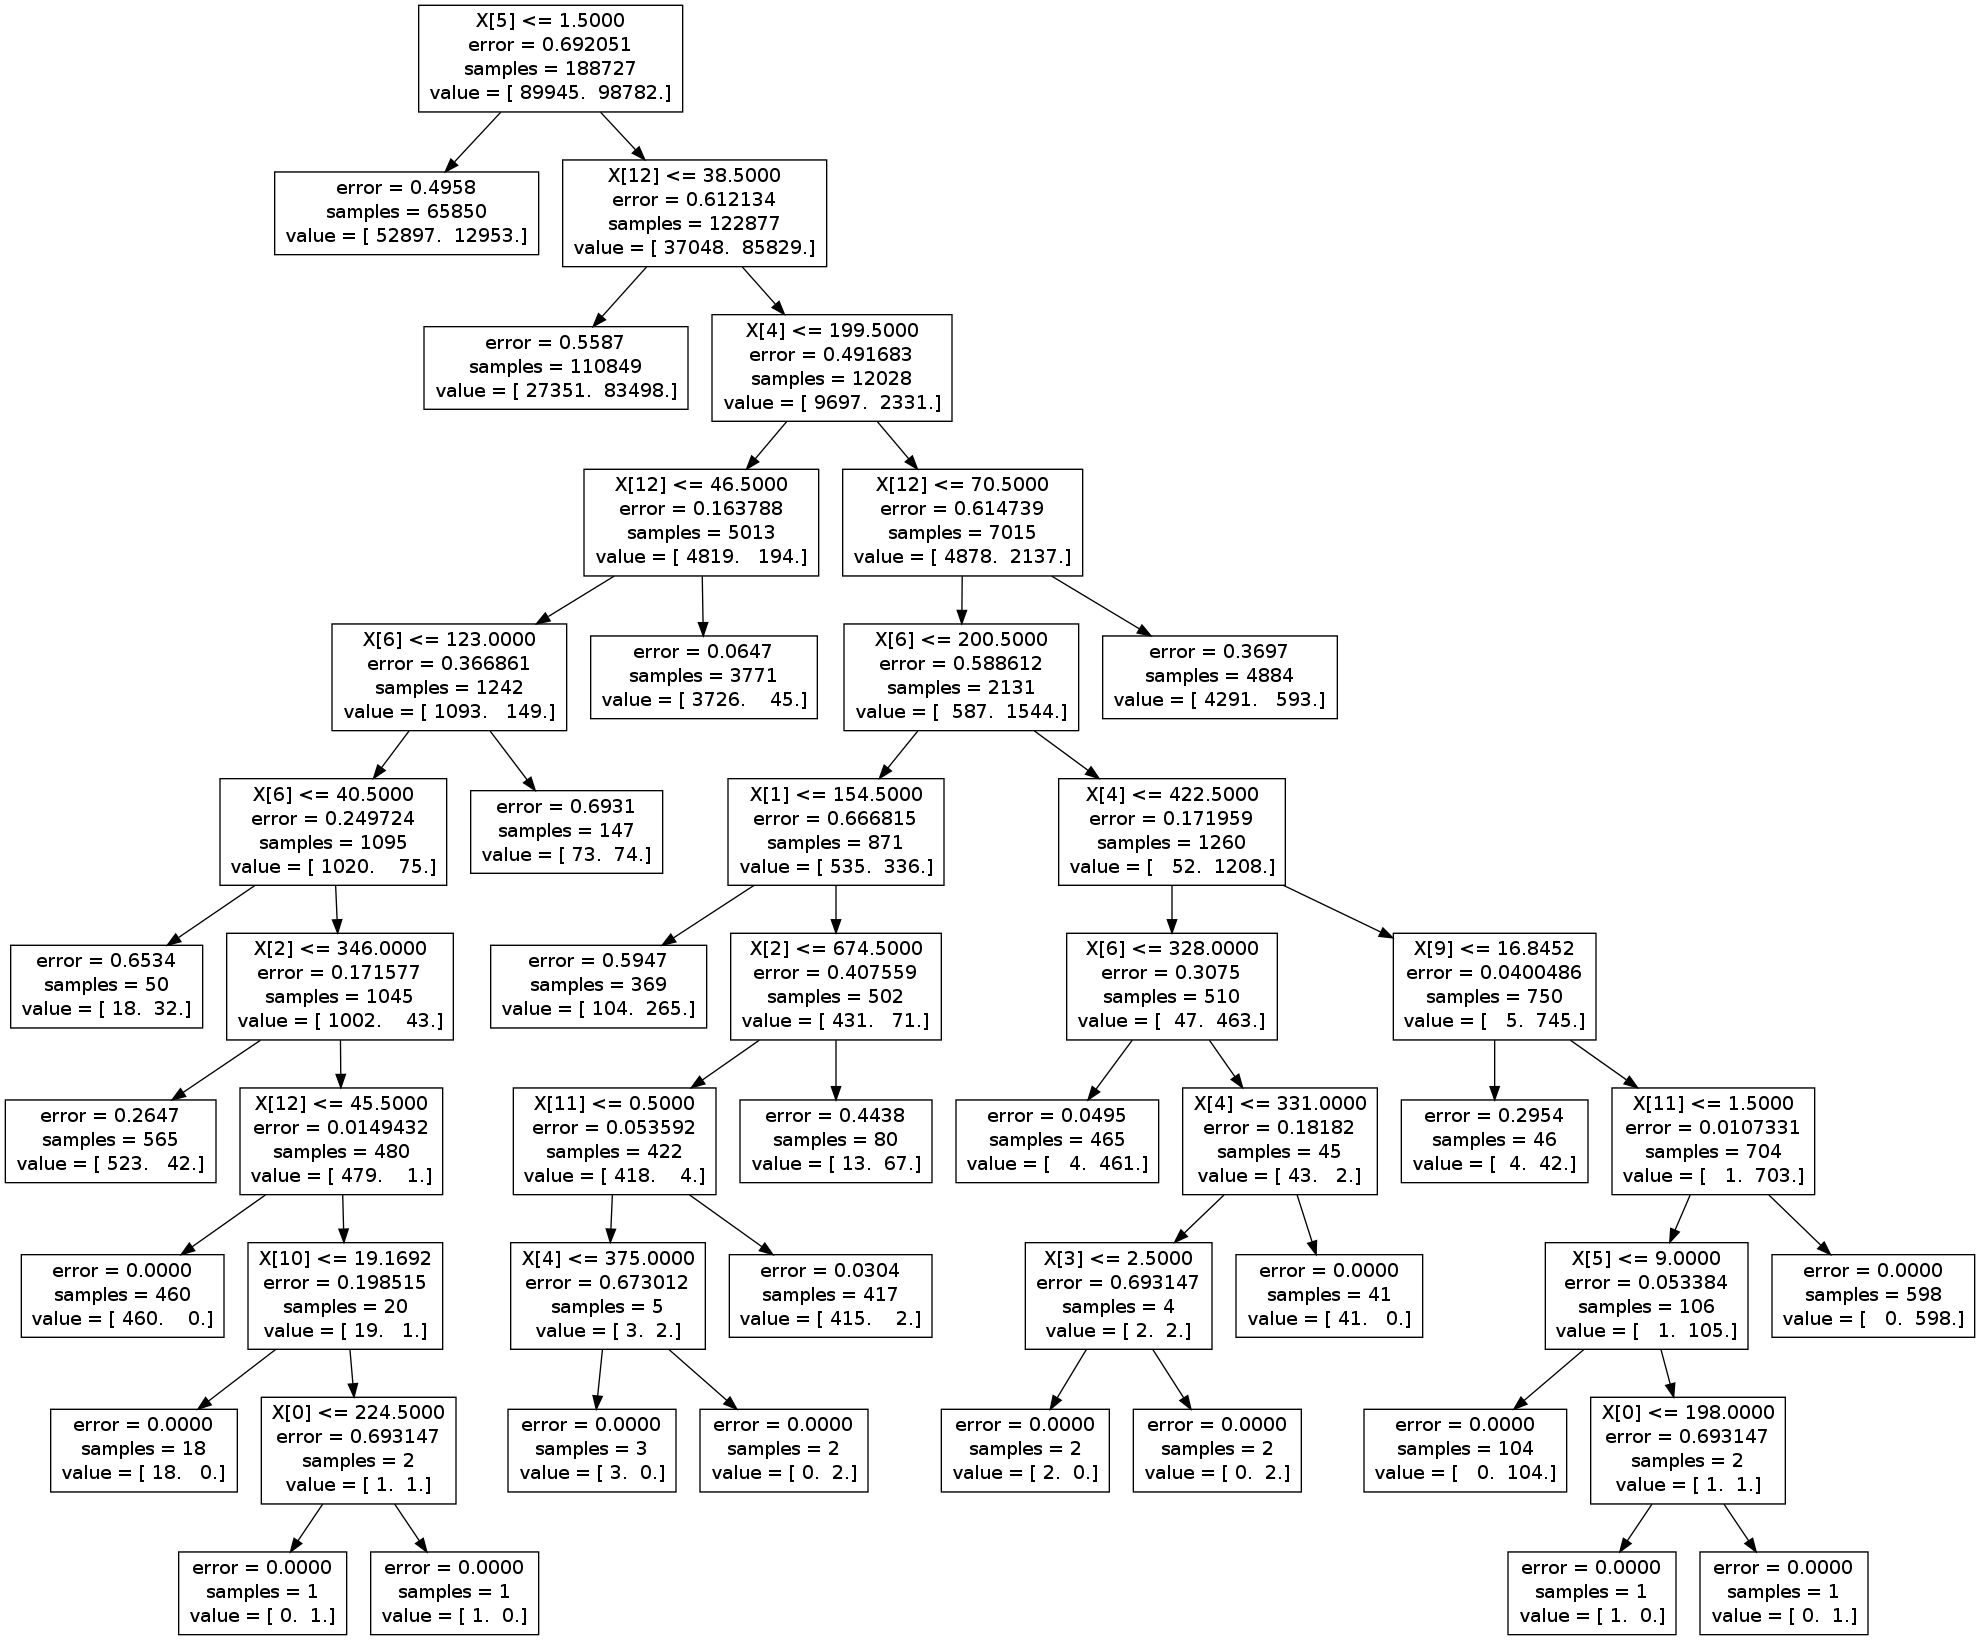
\includegraphics[width=\textwidth]{boss.png}
\caption{Pruned tree with 25 terminal nodes and max depth of 10.}\label{fig:tree}
\end{figure}

\subsection{Bagging and Boosting}

Bagging and boosting methods are known to increase performance of classifiers. We used random forest classifier as our bagging method and adaboost as our boosting method. We experimented with unbounded as well as fixed depth decision trees, keeping maximum depth of the tree at 10 (see section \ref{subsec:dectreemaxdepth}). 

For random forest, we vary number of trees by 10 over a range of 10 to 100. More than hundred trees are computationally expensive for a large dataset like ours, moreover, the difference in accuracy results are not significant. In general, our observation is that, for this dataset, improvements in performance are minor when using random forests. One intuitive reason might be that for our dataset number of features $<<$ number of data points and the random forests end up doing a sampling of the limited feature space.

For the performance of the random forests with unbounded and depth bounded trees, please refer to figure \ref{fig:randomforestunbounded}  and figure \ref{fig:randomforestbounded}, respectively. One interesting point to note is that when we use bounded depth trees, the single decision tree performs better than the random forest.

\begin{figure}[ht!]
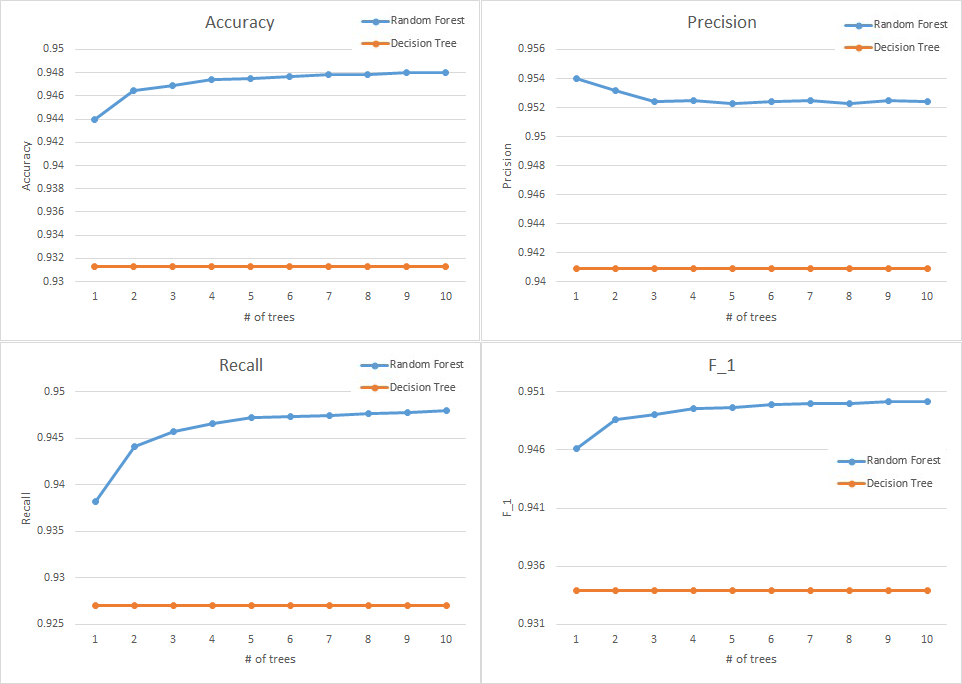
\includegraphics[width=\textwidth]{RF.png}
\caption{Random forest result with increasing number of unbounded depth  trees.}\label{fig:randomforestunbounded}
\end{figure}

\begin{figure}[ht!]
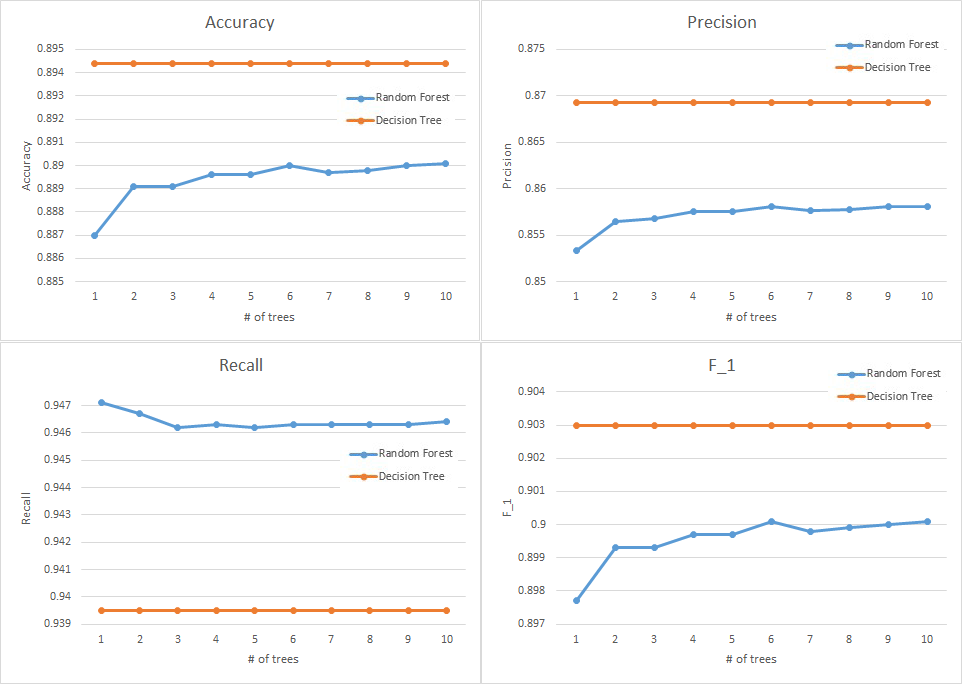
\includegraphics[width=\textwidth]{RF_Bounded.png}
\caption{Random forest result with increasing number of trees upto depth 10.}\label{fig:randomforestbounded}
\end{figure}

For adaboost, we report the results in table \ref{table:adaboost}. As adaboost is computationally very expensive, we can only compare the results of decision tree and adaboost for maximum tree depth=10 (we tried running adaboost with unbounded depth tree and it did not finish in more than one hour). For the bounded depth tree, adaboost shows significant improvements in all accuracy metrics. 

\begin{table}[ht!]
\centering
\caption{Performance improvement by adding adaboost to a decision tree of depth 10. }\label{table:adaboost}

\begin{tabular}{|l|c|c|}
\hline
& Without adaboost & With adaboost\\\hline
Accuracy & 0.8944 & 0.9507\\\hline
Precision (sensitivity) & 0.8693 &  0.9547\\\hline
Recall & 0.9395 & 0.9509\\\hline
F1 & 0.9030 & 0.9528\\\hline
\end{tabular}
\end{table}
%0.9507, 0.9547, 0.9509,
\section{Conclusions}
We applied decision trees, pruned decision trees, random forests and adboosting to the author attribution problem using data from the 2013 KDD Cup. We investigated the split and stopping criteria of the decision trees and found that information gain (entropy) works better than gini. Furthermore, we found that larger tree depths led to better performance; however, beyond some point this improvement was neglible and the models also became increasingly complex.

When we evaluated the effect of pruning the decision trees and plotted the accuracy against the number of leaves we found no evidence of overfitting taking place.

We found that overall adaboosting works the best, however it's very computationally expensive. Random forest also acheive improvements over standard unbounded decision trees for all evaluation metrics. However, because we have limited features this improvement is not that great.

%So that one takeaway lesson from this project is that for the scenario p $<<$ n (number of features is less and number of data points is large) one should use boosting methods over bagging methods. 
%\bibl iographystyle{plain}
%\bibliography{bibliography}



\end{document}